\section{Architecture and a Testable Adaptive Extension}
\label{sec:adaptive-extension}

This section specifies a successor, not an additional capability of the
evaluated bank. Figure~\ref{fig:layered-architecture} separates the implemented
physical estimator, proposed adaptation, and an external cyber layer.
Adaptive covariance estimation already appears in power-system dynamic
state estimation, including an IEEE-39 study \cite{wang2019adaptiveh}.
The question here is whether adaptation can follow instrumental changes
without explaining away a load or line intervention during recovery.

\begin{figure*}[t]\centering
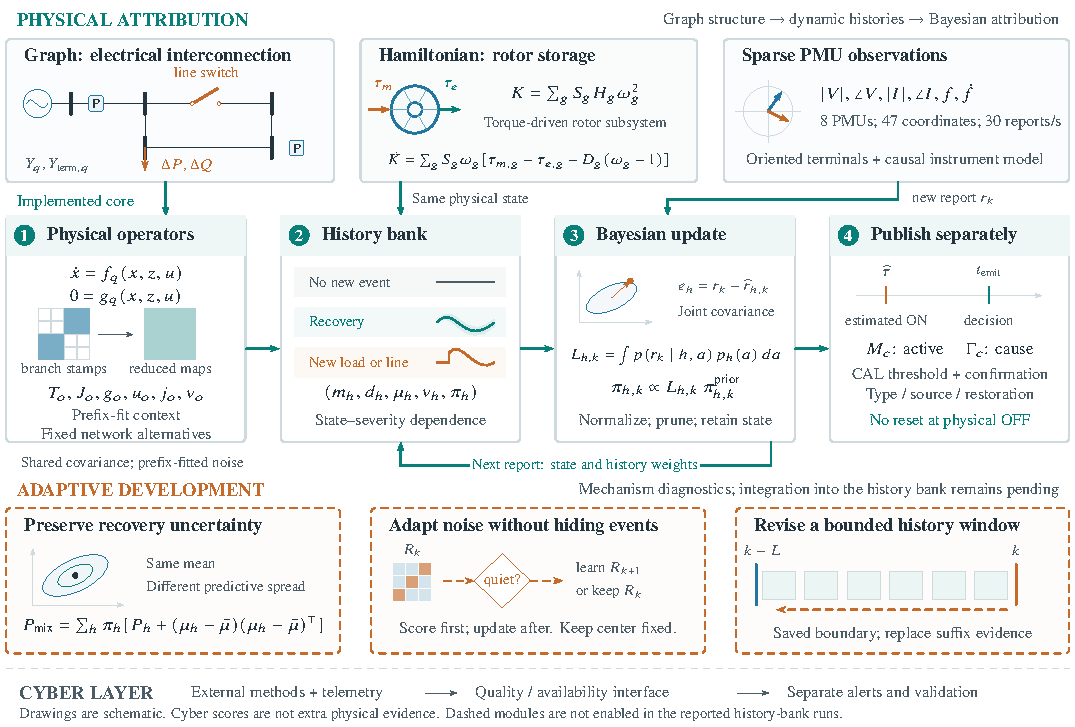
\includegraphics[width=.98\textwidth]{figures/generated/layered_architecture.pdf}
\caption{System architecture and implementation boundary. The solid upper path
is the reported physical bank. Dashed modules specify an unvalidated successor:
history-specific uncertainty, guarded noise adaptation and bounded-window
smoothing. The lower layer hosts separate cyber methods and outputs; neither
cyber scores nor nominal source-separation diagnostics are extra physical
likelihood factors. An availability interface requires a separately validated
measurement model.}
\label{fig:layered-architecture}
\end{figure*}

\subsection{Conditional Filtering Without Losing Severity Dependence}
For a fixed history, use the conventional predict--observe convention
$\xi_k=F_h\xi_{k-1}+c_h+B_ha+w_k$ and
$r_k=H_h\xi_k+d_h^{\rm obs}+D_ha+v_k$.
Assume independent zero-mean Gaussian process and observation noise,
constant severity within the history, and covariance independent of severity.
These timing conventions differ from the implemented combined one-report
operators; the equations are not a drop-in replacement for that code.
If $\xi_{k-1}\mid a,h,\mathcal F_{k-1}\sim
\mathcal N(m^++d^+a,P^+)$, the prediction is
\begin{align}
 m^-&=F_hm^++c_h,& d^-&=F_hd^++B_h,\nonumber\\
 P^-&=F_hP^+F_h^\top+Q_h.\label{eq:adaptive-affine-predict}
\end{align}
With $e=r_k-H_hm^--d_h^{\rm obs}$ and $s=H_hd^-+D_h$,
\begin{align}
 S&=H_hP^-H_h^\top+R_k,\quad K=P^-H_h^\top S^{-1},\nonumber\\
 m^+&=m^-+Ke,\quad d^+=d^--Ks,\nonumber\\
 P^+&=(I-KH_h)P^-(I-KH_h)^\top+KR_kK^\top.
 \label{eq:adaptive-affine-update}
\end{align}
The severity density is updated using $\mathcal N(e;sa,S)$ and the
same normalized truncated-Gaussian integral as the main method.
Its posterior variance $V_a$ contributes $d^+V_a(d^+)^\top$ to the
marginal state covariance. Substituting only the severity mean would lose
this dependence. At fusion, within-history and between-history covariance
must both be retained. Correlated process/observation errors require the
corresponding cross terms; merely changing $R$ in these equations is insufficient.

For an exogenous availability selector $E_k$, the admitted observation is
$E_kr_k$, with operators $E_kH_h,E_kD_h$ and covariance
$E_kR_kE_k^\top$. Missing values are marginalized, not replaced by zero
or held as independent new reports. In particular, taking a submatrix of
$R_k^{-1}$ generally gives the wrong marginal precision. An informative,
signal-dependent mask needs a selection model. The reported bank does not
yet implement this general interface.

\subsection{Learn Noise After Scoring the Current Report}
The first adaptive successor should fix $Q$, physical parameters and
the observation center. In fixed scaled observation coordinates, use
\begin{align}
 R_k&=U\operatorname{diag}(\lambda_k)U^\top+
       \operatorname{diag}(\delta_k),\nonumber\\
 &\lambda_k\ge0,\quad\delta_k\ge\delta_{\min}>0,
 \label{eq:adaptive-noise-family}
\end{align}
with fixed factor directions $U$, upper bounds and regularization selected
on development data. Common reference and local sensor errors motivate
these components; their factors are not freely identifiable in every
PMU layout. Instrument transformations must act on the full covariance;
temporally colored noise needs explicit states or a consistent whitening
model, not an instantaneous $R$ alone.

Let $\nu_r=r_r-\widehat r_{r\mid r-1}$ be a pre-correction innovation and
$C_r^{\rm pred}$ the nonmeasurement part of its predictive covariance.
For a mixture, $C_r^{\rm pred}$ includes severity uncertainty and the
spread of predictive means, not only $H_hP^-_hH_h^\top$.
A candidate covariance-matching update is
\begin{align}
 \widehat R_k^{\rm raw}
 &=\frac{\sum_{r\in W_k}\omega_r
       (\nu_r\nu_r^\top-C_r^{\rm pred})}{\sum_{r\in W_k}\omega_r},\nonumber\\
 R_{k+1}&=\Pi_{\mathcal R}!\left[(1-\eta)R_k+
                          \eta\widehat R_k^{\rm raw}\right].
 \label{eq:adaptive-noise-update}
\end{align}
If no eligible reports exist, retain $R_k$. Projection is a constrained
fit to the positive-definite family, not unrestricted eigenvalue clipping.
For example, bounded least squares on the fixed PSD factor matrices
preserves that family. The identity
$\mathbb E[\nu_r\nu_r^\top]=C_r^{\rm pred}+R_r$ requires a correctly
specified, conditionally centered predictor. A finite gated window need
not satisfy it; bias or unmodeled recovery can inflate the estimated noise.
Updating covariance must change both the quadratic score and its log
determinant, as well as the gain. Score report $k$ with $R_k$ before
allowing it to influence $R_{k+1}$.

Eligibility should depend on a sustained quiet-history state available
before the report, independent quality metadata, and a declared recovery
cooldown. This is an operational gate on approximate masses, not known
event truth. Selection by the current residual is dangerous: for
$Z\sim\mathcal N(0,1)$,
\begin{equation}
 \mathbb E[Z^2\mid |Z|<c]
 =1-\frac{2c\phi(c)}{2\Phi(c)-1}<1.
 \label{eq:adaptive-selection-bias}
\end{equation}
Thus retaining only small innovations underestimates variance even in
a correct model. Past-only eligibility avoids this particular current-report
truncation under the stated independence assumptions; it does not guarantee
that a weak or sustained intervention will be recognized. The design must
also test noise increases that make the gate stop admitting data.

Adapting the baseline can erase the event itself. If
$b_{k+1}=(1-\eta)b_k+\eta a$, $b_0=0$, then before the next update
$a-b_k=a(1-\eta)^k$. This elementary counterexample motivates keeping
the center fixed in the first successor. Continuous impedance or operating
parameter adaptation remains deferred until its effect can be separated
from event severity; learning unrestricted $Q$, $R$ and parameters together
does not establish their identifiability.

\subsection{Historical Revision and Separate Cyber Outputs}
A bounded-window smoother needs a saved boundary distribution and a
record of the covariance/parameter version used for each report.
For the same boundary model, replace the old suffix by the recomputed
one, $\log W_h^{\rm new}=\log W_h^{\rm old}
-\ell_{h,W}^{\rm old}+\ell_{h,W}^{\rm new}$.
Changing the boundary model instead requires rebuilding its contribution.
Replaying a suffix must not rerun the adaptation learner or count its
observations again. Revised historical estimates are published at the
current report time; earlier alarms remain in the audit log.
Unlike the current split inner/outer replay, a coherent successor must
update both levels consistently or declare the remaining approximation.
Plug-in $\widehat R_k,\widehat\theta_k$ do not constitute a joint Bayesian
posterior over those parameters.

The external cyber layer consumes its own telemetry and metadata and
emits separately evaluated alerts. Missing or corrupted PMU reports do
not establish a cyber attack. A quality flag may enter a declared
measurement-selection rule; an attack score is not another independent
likelihood of the same phasors. Simultaneous physical and integrity
changes require paired tests of that interface.

\subsection{Verification and Evidence Still Required}
The bundled numerical verification checks the
affine update and severity integral against numerical quadrature, the
Joseph covariance against Gaussian conditioning, structured covariance
projection, missing-coordinate marginalization, prefix invariance and
suffix replacement on a small adaptive Gaussian model. It also verifies
the two counterexamples above. These are numerical checks of the proposed
building blocks, not load-attribution or false-alarm results.

A fresh campaign should first compare fixed shared covariance with
history-specific covariance, then add structured noise adaptation with
and without the history gate. Test smoothing and memory compression
separately. Each arm needs independent calibration to the same normal-alarm
target, with infeasible arms declared. Include independent PMU noise,
normal noise changes, long weak interventions, recovery, parameter shift
and missing reports. Freeze settings and parents before TEST; compare
timely attribution, extra alarms, normal exposure, predictive score,
availability and latency by parent. Neither this design nor its numerical
checks modify the ongoing campaigns or establish superiority of the adaptive extension.
